A preliminary step is to find a suitable robot platform that enables both the development and testing of indoor aerial SLAM methods.
A straightforward choice is to use a \textit{quadrotor helicopter}, commonly designed to be unmanned aerial vehicles (UAVs).
Their small size and extremely maneuverability allows both indoor and outdoor flights.
Furthermore, quadrotors do not require mechanical linkages to vary the rotor blade pitch angle, which simplifies the design.

Nowadays, small quadrotors with on-board stabilization can be bought off-the-shelf.
These quadrotors make it possible to shift the research from basic control of the platform towards intelligent applications.
The platform selected is the Parrot AR.Drone\footnote{\url{http://ardrone.parrot.com}} quadrotor helicopter.
The main advantages of this quadrotor are its robustness and affordable pricetag.
The AR.Drone is equipped with a front-camera and a down-looking camera that provide live video streaming.
Two complementary algorithms make use of the down-looking camera for improved stabilization.
Furthermore, the AR.Drone is equipped with an ultrasound sensor and an inertial unit that measures pitch, roll, yaw and accelerations along all axes.
The vehicle is controlled by sending commands over a Wi-Fi connection.

In this chapter, the AR.Drone is evaluated as a robotic platform.
The flight control of a quadrotor is described, AR.Drone's hardware is listed and the intelligent onboard software is described.
Moreover, the open Application Programming Interface (API) is examined.


% Quadrotor flight control
\section{Quadrotor flight control}
\label{sec:platform-quadrotor-flight-control}

\begin{figure}[htb]
\centering
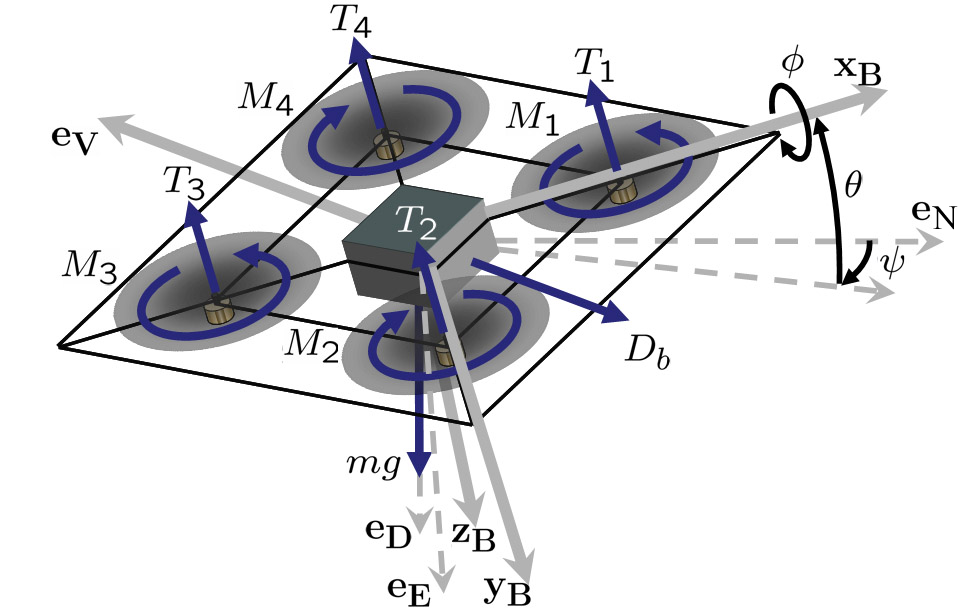
\includegraphics[width=8cm]{images/QuadRotorBody.png}
\caption{Free body diagram of a quadrotor helicopter 
(Courtesy Hoffman \textit{et al.} \cite{Hoffmann2007}). Note that a right-handed orthogonal coordinate system is used with the $z$-axis pointing down. Each of the 4 motors has a thrust $T_i$ and momentum $M_i$. Together the motors should generate sufficient vertical thrust to stay airborne, which is indicated by the gravity force $mg$ in the direction $e_D$. Differential thrust between the motors can provide roll $\phi$ and pitch $\theta$ torques, which lead to an angle of attack $\alpha$. This can result in fast movements of the helicopter (e.g. in the horizontal plane) in the direction $e_V$ which a resulting drag force $D_b$. }
\label{fig:QuadRotorBody}
\end{figure}

% http://www.stanford.edu/~haomiao/papers/ICRA09AeroEffects.pdf
% http://www2.engr.arizona.edu/~sprinkjm/research/c2wt/uploads/Main/QuadrotorDynamicsGNC.pdf
The mechanical structure of a quadrotor consists of four rotors attached to a body frame (see Figure \ref{fig:QuadRotorBody}).
Each pair of opposite rotors (pair ${1, 3}$ and pair ${2, 4}$) is turning the same direction.
One pair is turning clockwise and the other counter-clockwise.
Each rotor produces both a thrust $T$ and torque $\tau$ about its center of rotation, as well as a drag force $D_b$ opposite to the vehicle's direction of flight.
\textit{Thrust} $T$ is a force that is generated by expelling or accelerating mass in one direction.
The accelerated mass will cause a force of equal magnitude but opposite direction on that system.
\textit{Torque} $\tau$ is the tendency of a force to rotate an object about an axis.
\textit{Drag} $D_b$ is the force that opposes the motion of an aircraft through the air.
This force depends on velocity of the vehicle and de-accelerates the vehicle if insufficient thrust is generated.
Together the motors should generate sufficient vertical thrust to stay airborne, which is indicated by the gravity force $mg$ in the direction $e_D$.

\begin{figure}[htb]
\centering
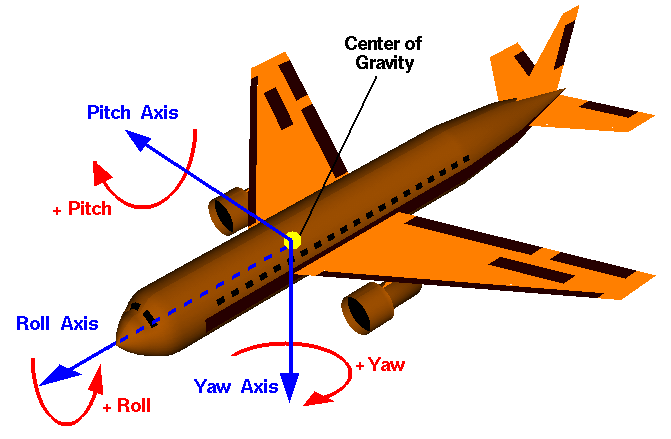
\includegraphics[width=8cm]{images/Rollpitchyawplain.png}
\caption{Roll, yaw and pitch axis orientation for an aerial vehicle.}
\label{fig:roll-pitch-yaw}
\end{figure}

For movements, the quadrotor relies %solely
on differential torque and thrust.
\textit{Pitch}, \textit{roll} and \textit{yaw} are used in flight dynamics to indicate the angles of rotation in three dimensions about the vehicle's center of mass (see Figure \ref{fig:roll-pitch-yaw}).
If all rotors are spinning at the same angular velocity, the differential torque is zero, resulting in no angular acceleration about the yaw axis.
Varying the angular velocity of each rotor pair yields angular acceleration about the yaw axis.
If the total thrust is kept constant, the vertical velocity remains unchanged.
A vertical movement is achieved by increasing or decreasing the thrust from each motor by the same amount, so that total thrust changes but differential torque on the body remains zero. 
A horizontal movement is achieved by maintaining a non-zero pitch $\theta$ or roll angle $\phi$.
Angular accelerations about the pitch and roll axes can be generated separately.
Each pair of blades rotating in the same direction controls one axis, either roll or pitch.
Increasing thrust for one rotor while decreasing thrust for the other will maintain the torque balance needed for yaw stability and induce a differential torque about the roll or pitch axes. 

%\section{Hardware}
\begin{comment}
\begin{figure}[htb]
\centering
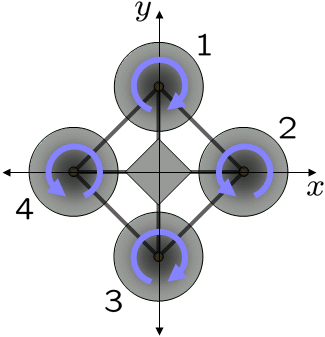
\includegraphics[width=7cm]{images/Quadrotor_yaw_torque.png}
\caption{Schematic of reaction torques on each motor of a quadrotor helicopter. Rotors 1 and 3 spin in one direction, while rotors 2 and 4 spin in the opposite direction, yielding opposing torques for control.}
\label{fig:QuadRotorRotors}
\end{figure}
\end{comment}

% Hardware
\section{Hardware}
\begin{figure}[htb]
\centering
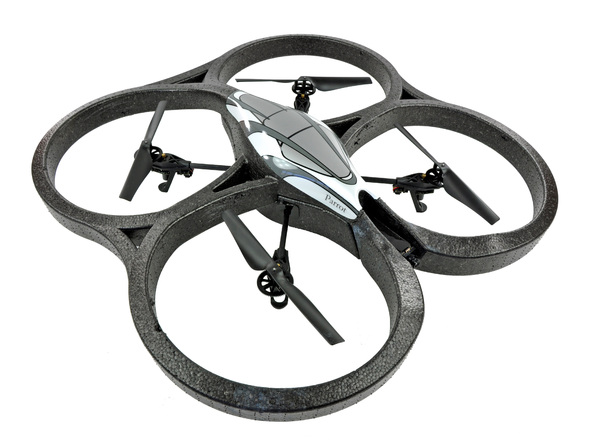
\includegraphics[width=9cm]{images/ardrone.jpg}
\caption{The AR.Drone quadrotor helicopter with protection hull attached.}
\label{fig:ardrone_hull}
\end{figure}
The AR.Drone (Figure \ref{fig:ardrone_hull}) is a remote-controlled consumer quadrotor helicopter developed by Parrot SA\footnote{\url{www.parrot.com}}.
The body is made of a carbon fiber tube structure and high resistance 
%PA66
plastic.
A protection hull is made of Expanded Polypropylene (EPP) foam\footnote{\url{http://en.wikipedia.org/wiki/Polypropylene}}, which is durable, light in weight and recyclable.
The hull provides protection during indoor flights.
The propellers are powered by four brushless motors (35,000 rpm, power: 15W).
Energy is provided by a Lithium polymer battery with a capacity of 1000 mAh, which allows a flight time of approximately 10 minutes.

The AR.Drone carries an internal computer with a 468MHz ARM9-processor and 128MB of RAM, running a custom Linux operating system.
A mini-USB connector is included for software flashing purposes and to attach add-ons (e.g., GPS sensor).
An integrated 802.11g wireless card provides network connectivity with an external device that controls the vehicle.
A remote control is not included. Instead, a regular WiFi-enabled device can be used to control the AR.Drone.
The AR.Drone was initially designed for Apple platforms (e.g., iPhone, iPod and iPad) and became available on other platforms during 2011.
It is also possible to control the AR.Drone from a Linux or Windows PC with the software designed for application developers.



% Sensors
\subsection{Sensors}
The AR.Drone has different types of sensors.
These sensors are used for automatic stabilization.
In addition, a front camera provides the user with visual feedback from the vehicle.


\subsubsection{Inertial measurement unit}
The AR.Drone features a 6 degrees of freedom (DOF) inertial measurement unit.
It provides the onboard software with pitch, roll and yaw measurements.
%Pitch, roll and yaw are often used in flight dynamics and indicate the angles of rotation in three dimensions about the vehicle's center of mass.
These measurements are used for automatic pitch, roll and yaw stabilization and assisted tilting control.
The measurement unit is a \textit{micro electro-mechanical system} (MEMS) and contains
a 3 axis accelerometer, a 2 axis roll and pitch gyrometer and a single axis yaw gyrometer.

The \textbf{accelerometer} is a BMA150\footnote{\url{http://www.bosch-sensortec.com/content/language1/downloads/BMA150_DataSheet_Rev.1.5_30May2008.pdf}} made by Bosch Sensortec.
%It provides three sensitivity ranges (i.e., maximum g-force it can report): $\pm 2g / \pm 4g / \pm 8g$.
An accelerometer outputs g-forces (acceleration relative to free-fall) as a quantity of acceleration.
It is based on the phenomenon that the (observed) weight of a mass changes during acceleration.
A typical MEMS accelerometer is composed of movable \textit{proof mass} with plates that is attached through a mechanical suspension system to a reference frame.
Movable plates and fixed outer plates represent capacitors. The deflection of proof mass is measured using the capacitance difference.
The accelerometer has three perpendicular axes. Each axis can only measure acceleration in the direction of the axis.
%The tiny micro-structures can only measure force in a single direction, or axis of acceleration.
%This means with a single axis measured, you can only know the force in either the X, Y, or Z directions.
An accelerometer at rest relative to the Earth's surface will indicate approximately 1 g upwards, because any point on the Earth's surface is accelerating upwards relative to the local inertial frame.
To obtain the acceleration due to motion with respect to the Earth, this gravity offset must be subtracted and corrected for effects caused by the Earth's rotation relative to the inertial frame.
Since the accelerometer can measure gravity, it can be used as a tilt sensor.

The AR.Drone has a 2 axis roll and pitch \textbf{gyrometer} and a single axis yaw gyrometer.
The gyrometer measures angular velocity in degrees per second, based on the principles of angular momentum.
In order to estimate the absolute angle $\theta$, the angular velocity signal $\Omega$ needs to be integrated with respect to time.
A major problem with this method is that bias errors in the angular velocity signal will cause the integrated angle value to drift over time, since all gyroscopes have at least a small amount of bias error in their angular rate signal.

Regular gyroscopes use a spinning wheel.
However, a small device like the AR.Drone cannot afford to have a spinning wheel.
Instead, a tiny MEMS gyroscope is used. 
%In a MEMS gyroscope, two proof masses vibrate in plane at certain frequency.
It comprises of a plate, called the \textit{proof mass}, that vibrates (oscillates).
%when a drive signal is applied to set of drive capacitor plates.
When the vehicle rotates, the proof mass gets displaced in the $x$, $y$, and $z$ directions by Coriolis forces.
A processor senses the proof mass’ displacement through capacitor plates located underneath the proof mass, as well as finger capacitors at the edges of the package.
The AR.Drone uses a IDG-500 Dual-Axis\footnote{\url{http://www.sparkfun.com/datasheets/Components/SMD/Datasheet_IDG500.pdf}} gyroscope for the pitch and roll angles of the drone.
The IDG-500 gyro has two separate outputs per axis for higher speed motions (range: $500^{\circ}/s$, sensitivity: $2.0mV/^{\circ}/s$) and lower-speed precise movements (range: $110^{\circ}/s$, sensitivity: $9.1mV/^{\circ}/s$).
The yaw orientation is measured using a high precision gyrometer, the Epson Toyocom XV-3500CB\footnote{\url{http://www.eea.epson.com/portal/pls/portal/docs/1/424992.PDF}}.
This sensor has a range of $100^{\circ}/s$ and a sensitivity of $0.67mV/^{\circ}/s$.
%Vibrating structure gyroscopes are simpler and cheaper than conventional rotating gyroscopes of similar accuracy
%The output is a rate of rotation about the X and Y axis.


\subsubsection{Ultrasound altimeter}
\label{sec:ultrasound_altimeter}
An ultrasound sensor provides altitude measures for automatic altitude stabilization and assisted vertical speed control.
The ultrasound sensor is attached on the bottom of the AR.Drone and points downward in order to measure the distance to the floor.
A packet of ultrasonic soundwaves is transmitted towards the floor, which reflects the sound back to the sensor.
The system then measures the time $t$ for the echo to return to the sensor and computes the distance $d$ to the target using the speed of sound:
\begin{equation}
d = \frac{c \times t}{2}
\end{equation}
where $c \approx 343\small{m/s}$ is the speed of sound in air.

Ultrasound range measurements suffer from some fundamental drawbacks which limit the usefulness.
These drawbacks are inherent to the principle of an ultrasonic sensor and their commonly used wavelengths.
Borenstein and Koren \cite{borenstein1988obstacle} describe some of these drawbacks in the context of obstacle avoidance.
A limitation is the small range in which the sensor is able to operate.
The ultrasound sensor in the AR.Drone has an effective range of approximately $20\small{cm}$ to $6\small{m}$.
%The minimum range is approximately $20\small{cm}$, meaning that the AR.Drone is \textit{unable to determine its altitude} when flying close to the floor.
Another limitation is that the ultrasound sensor is unable to obtain precise directional information about objects.
Sound propagates in a cone-like manner, where opening angles are commonly between $20$ to $40$ degrees.
Due to this property, the sensor acquires entire regions of constant depth instead of discrete depth points.
So, the ultrasound sensor can only tell there is an object at the measured distance somewhere within the measured cone.

Another limitation is the influence of the surface's orientation on the sensor's performance.
When the ultrasoundwave is emitted toward a parallel surface of an obstacle, most of the sound energy is reflected perpendicular to the surface and will be detected by the sensor.
However, if the surface of the obstacle is tilted relative to the sensor, then only an undetectably small amount of energy will be reflected toward the sensor.
Also, the acoustic properties of the material in range have direct impact on the sensor's performance (e.g., foam can acoustically absorb the soundwaves).
A final limitation is the limited operating frequency.
Before a soundwave can be emitted, the previously emitted soundwave has to be detected by the sensor.
This reduces the minimal operating speed of the AR.Drone's ultrasound sensor to $300 / (2 \times 6) = 25\small{Hz}$.

The opening angle of the AR.Drone's ultrasound sensor is not documented.
Appendix \ref{appendix:opening_angle} describes an experiment that was performed to determine the opening angle.
The average opening angle was determined as $25.03^{\circ}$ with a standard deviation of $1.45^{\circ}$.

During flight, the AR.Drone can take a broad range of angles\footnote{The AR.Drone's default maximum angle of attack is $12^{\circ}$}.
The floor is not always perpendicular to the orientation of the ultrasound sensor, which may influence the altitude measurements.
A small experiment was performed to measure the effect of the AR.Drone's angle of attack $\alpha$ and the error $\epsilon$ of the measured altitude.
This experiment was performed above a flat floor.
The angle of attack $\alpha$ was changed slowly while keeping the AR.Drone at a fixed altitude.
A relation between the angle $\alpha$ and measured altitude was observed.
The following (first degree) polynomial fit describes the relation between the angle $\alpha$ in degrees and error $\epsilon$ of the measured altitude:
\begin{equation}
\epsilon = 0.2214 \times \alpha \hspace{0.2cm} \begin{small}cm\end{small}
\end{equation}
\normalsize
\normalcolor



\subsubsection{Cameras}
The AR.Drone is equipped with two CMOS cameras: a front camera and a bottom camera.
Both cameras support live video streaming at 15 frames per second.

The front camera has a resolution of $640 \times 480$ pixels (VGA) and a wide $93^{\circ}$ field of view.
This front camera is used to automatically detect other drones during multiplayer games or to provide video feedback on a screen (e.g., smartphone).
The bottom camera has a resolution of $176 \times 144$ pixels (QCIF) and a $64^{\circ}$ field of view.
The video frequency of this camera is 60 frames per second to reduce motion blur and improve the applicability of intelligent algorithms.
Despite the high frequency, the frames are streamed at 15 frames per second.

%\textit{front + bottom camera sample}

The bottom camera plays a central role in the AR.Drone's onboard intelligence.
It is used for horizontal stabilization (i.e., automatic hovering and trimming) and to estimate the velocity of the drone.
More details about the onboard intelligence can be found in Section \ref{sec:platform_onboard_intelligence}.



% Onboard intelligence
\section{Onboard intelligence}
\label{sec:platform_onboard_intelligence}
Usually quadrotor remote controls have multiple joysticks and knobs for controlling pitch, roll, yaw and throttle.
It generally takes hours of practice to safely perform basic maneuvers like take-off, trimming, hovering with constant altitude and landing.
Thanks to the onboard computer and sensors, take-off, hovering, trimming and landing are now completely automatic and all maneuvers are assisted.

Because the quadrotor system is unstable, feedback from the sensors to the control system is required.
This raises the issue of state estimation.
The vehicle's control system must be robust to cope with various disturbances that can be encountered in practice.
Redundancy in the state estimation is the solution in this case.
The AR.Drone has multiple methods to compute estimated states.
However, the onboard software (firmware) is closed source and not documented by the manufacturer.
In August 2011, the manufacturer's academic partner \textit{MINES ParisTech for navigation and control design}, published an article \cite{bristeau2011navigation} which globally describes the navigation and control technology inside the AR.Drone.



\subsection{Sensor calibration}
The AR.Drone uses low-cost sensors, which introduce issues like bias, misalignment angles and scale factors.
These errors are not negligible and differ between AR.Drones.
For this reason, a manual board calibration is performed at the factory.
This calibration process computes the unknown parameters using a least-square minimization method:
\begin{equation}
Y_m = AY_v + B
\end{equation}
where $Y_m$ is the measurement and $Y_v$ the true value of the sensed variable.

Not all errors are compensated during the factory calibration.
The AR.Drone's navigation board is mounted on damping foam.
To further compensate the misalignment, \textit{onboard calibration} is performed.
This is done by considering that the mean acceleration of the UAV must be equal to zero on a stationary flight.
A least-squares minimization method is used to determine the micro-rotation.
After each landing, this onboard calibration is automatically performed to compensate for the misalignment due to the displacement of the damping foam during the landing shock.

After inertial sensor calibration, sensors are used inside a complementary filter to estimate the attitude and de-bias the gyroscopes.
The de-biased gyroscopes are used for vision velocity information combined with the velocity and altitude estimates from a vertical dynamics observer.
The velocity from the computer vision algorithm is used to de-bias the accelerometers, the estimated bias is used to increase the accuracy of the attitude estimation algorithm.
Finally, the de-biased accelerometer gives a precise body velocity from an aerodynamics model.


\subsection{State estimation}
To address the problem of state estimation, the AR.Drone is equipped with embedded sensors that are described in the previous section.
When combining the sensor measurements in data fusion algorithms, relatively good state estimates are obtained.
Multiple techniques form a tightly integrated vision and inertial navigation filter that can be summarized as described hereafter.
After the inertial sensors are calibrated, the sensors are used inside a complementary filter to estimate the attitude and de-bias the gyroscopes.
The de-biased gyroscopes are used for vision-based velocity information provided by the vertical camera.
The vision-based velocity is used to de-bias the accelerometers. This estimated accelerometer bias is used to increase the accuracy of the attitude estimation algorithm.
Eventually, the de-biased accelerometer gives a precise body velocity from an aerodynamics model.
Below, some techniques are described in more detail.

\subsubsection{Visual odometry}
\label{sec:platform-visual-odometry}
The images provided by the vertical camera are used to estimate the 3D velocity of the vehicle.
This process is called Visual Odometry and is introduced in Section \ref{sec:background-visual-odometry}.
According to \cite{bristeau2011navigation}, two complementary algorithms are available.
Depending on the scene content or the expected quality of their results, one is preferred to the other.

The first algorithm is a multi-resolution scheme.
The methodology is described in \cite{lukas1981iterative}.
It computes the optical flow over the whole picture range using a kernel to smooth spatial and temporal derivatives.
Attitude changes between two images are ignored during the first resolution refinement step.
The error is finally efficiently canceled in most cases by subtracting the displacement of the optical center induced by the attitude change alone.
The second algorithm estimates the displacement of several interesting image points (features).
For this, FAST image features \cite{rosten2010faster} are used.
An iteratively weighted least-squares minimization procedure is used to recover the displacements.
The IRLS estimation \cite{michaelsen2004pose} is carried out by assuming the depth of the scene is uniform.
This optical flow based method is used by default.
When the scene is deemed suitable for the corner detector and the flight speed is low, the system switches to the second algorithm for increased accuracy.

The inertial sensors are used to compensate for the small rotation between consecutive camera frames.
This is a significant help for the determination of the optical flow in the vision algorithm.
A specific linear data fusion algorithm combining sonar and accelerometer information is implemented to give accurate vertical velocity and position estimates. % above the obstacle.

\subsubsection{Aerodynamics model}
Unfortunately, the vision-based velocity is noisy and relatively slowly updated compared to the vehicle dynamics.
The estimated velocity is improved with the help of an aerodynamics model.
The accelerometers and gyroscopes are used together as inputs in the motion dynamics to estimate the attitude and velocities.
When the aerodynamics velocity and the vision velocity are simultaneously available, the accelerometer bias is estimated and vision-based velocity is filtered.
Alternatively, when vision-based velocity is unavailable, only the aerodynamics estimate is used with the last updated value of the bias.

The dynamic behavior of a quadrotor is quite complex.
In particular, the aerodynamics of the propellers and the motion of the rigid frame can interfere to produce a coupled dynamical model.
This model is beyond the scope of this thesis.
In summary, linear drag term exists from the interaction between the rigid body and the rotors and this term is reinforced by tilt phenomenon, which changes a lift force component in drag.
These induced-drag effects are non-negligible and they yield interesting information on the velocity of the system.
The induced forces are directly measured by the accelerometers, and through the model, can be used to reliably estimate the velocities of the vehicle.

Section \ref{sec:pose_estimation} describes how the estimated velocities can be used to estimate the position of the AR.Drone.



\subsection{Controls}
\label{sec:platform-controls}
The AR.Drone performs actions based on the estimated state and the input from the pilot.
A pilot controls the linear and lateral velocity with an input signal $s$ that specifies the pitch of the drone as a factor (between 0 and 1) of the maximum absolute tilt $\theta_{max}$.
The altitude is controlled with an input signal that specifies the desired vertical speed as a factor (between 0 and 1) of the maximum vertical velocity $v_{max}$.
A finite state machine is used to handle different modes of the vehicle (e.g., flight, hovering, take off and landing).

The control is realized by two nested loops, the \textit{Attitude Control Loop} and the \textit{Angular Rate Control Loop}.
The Attitude Control Loop computes an angular rate from the difference between the estimated attitude and the desired attitude (which is based on the velocity requested by the pilot).
The angular rate is tracked with a Proportional Integral (PI) controller.
The Angular Rate Control Loop controls the motors with simple proportional controllers.
When no user input is given, the AR.Drone goes in hovering mode, where the altitude is kept constant and velocity is stabilized to zero.
Transition from flight mode to hovering mode is realized with a motion planning technique, designed to obtain zero speed and zero attitude in short time and without overshooting.
For this, a feed-forward control uses inversion of the governing dynamics.
The hovering mode is maintained by the Hovering Control Loop, which consists of a PI controller on the estimated speed.

The Attitude Control Loop is also responsible for altitude stabilization (i.e., maintaining a fixed distance between the floor and vehicle).
For this, feedback from the ultrasound sensor is used.
When an obstacle is in range of the ultrasound sensor, the measured altitude decreases.
The AR.Drone responds by increasing its absolute altitude to maintain a fixed measured altitude.
Consequently, the AR.Drone decreases its absolute altitude when the obstacle is out of range.
However, this behavior was not always observed during experiments.
For example, when a floating object ($70\small{cm}$ above the floor) becomes in range of the ultrasound sensor.
In these cases, the raw ultrasound measurements show a sudden large change, while the onboard filtered altitude measurements show a small change (Figure \ref{fig:platform-ultasound-raw-filtered}).
Now, AR.Drone does not change its absolute altitude and remains at the same absolute altitude.
This observation suggests that the altitude stabilization is based on a filtered derivative of the ultrasound measurements.
%\small{(raw measurements should cause convergence to the actual measurements over time)} of the raw ultrasound measurements.
The filter minimizes the impact of sudden changes that occur for a short period of time.

\begin{figure}[htb]
\centering
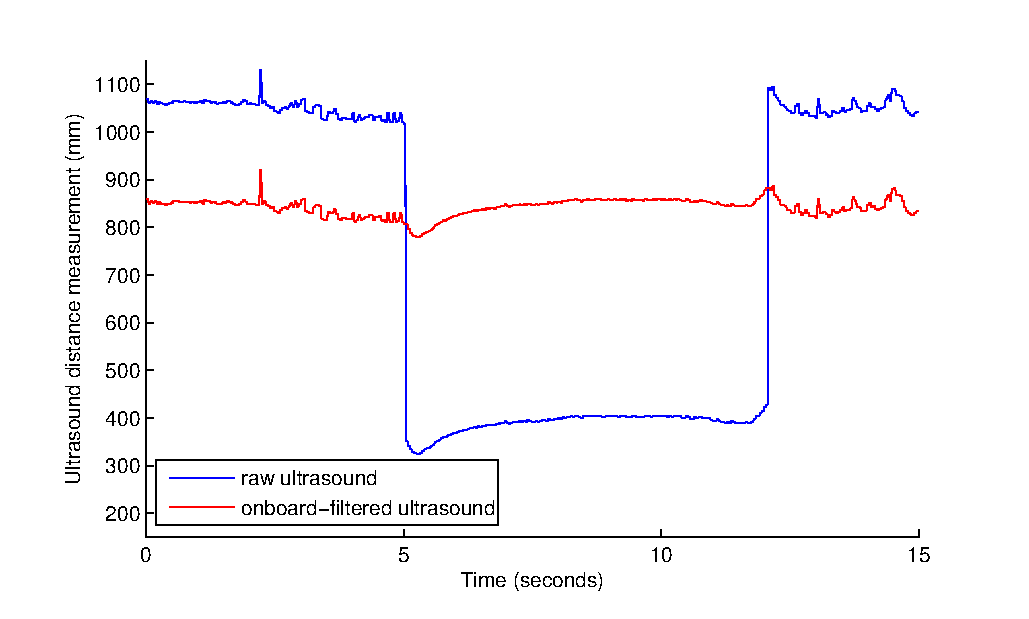
\includegraphics[height=6cm]{images/altitude_raw_vs_filtered_1m_obstacle.eps}
\caption{Comparison between the AR.Drone's raw and filtered ultrasound measurements when an object floating at  $1\small{m}$ comes in range of the ultrasound sensor.}
\label{fig:platform-ultasound-raw-filtered}
\end{figure}

Similar to altitude stabilization, the ultrasound sensor is used for take-off and landing.
When a take-off command is issued, the engines are started automatically and the AR.Drone increases its altitude until a pre-determined altitude is reached (which is $50\small{cm}$ by default). When this altitude is reached, the vehicle switches to hovering mode.
During the take-off procedure, the AR.Drone is likely to generate some (random) horizontal movements.
These movements are often not observed by the AR.Drone's internal state estimation, probably due to the bad lightning conditions for the vision-based algorithms.
In case of a landing command, the AR.Drone decreases its altitude until it has landed on the floor. The vertical velocity is decreased when the drone comes near the floor to prevent a heavy shock.
The engines are stopped automatically.

%\textit{Funny observation: sticking tape on the ultrasound sensor results in infinite take-off and landing (e.g., vehicle keeps increasing or decreasing altitude).}


% Open application programming interface
\section{Open Application Programming Interface}
\label{sec:API}
The AR.Drone API\footnote{\url{https://projects.ardrone.org}} (Application Programming Interface) is the reference project for developing applications for the AR.Drone.
It includes SDK (Software Development Kit) source code written in C, multiplatform examples and documentation.
The API does not include software that is embedded on the AR.Drone.

Communication with the AR.Drone is done through four main \textit{communication services}, which are implemented in the SDK.
\begin{enumerate}
\item Controlling and configuring the drone is done by sending \textit{AT commands} on regular basis;
\item Information about the drone (e.g., status, altitude, attitude, speed) is called \textit{navdata}.
The navdata also includes filtered and raw sensor measurements.
This information is sent by the drone to its client at a frequency of approximately $30$ (demo mode) or $200$ times per second;
\item A video stream is sent by the AR.Drone to the client device.
Images from this video stream are decoded using the codecs (decoders) included in the SDK.
\item Critical data is communicated over a channel called the \textit{control port}.
This is a TCP connection to provide reliable communication.
It is used to retrieve configuration data and to acknowledge important information such as the sending of configuration information.
\end{enumerate}

\begin{figure}[htb]
\centering
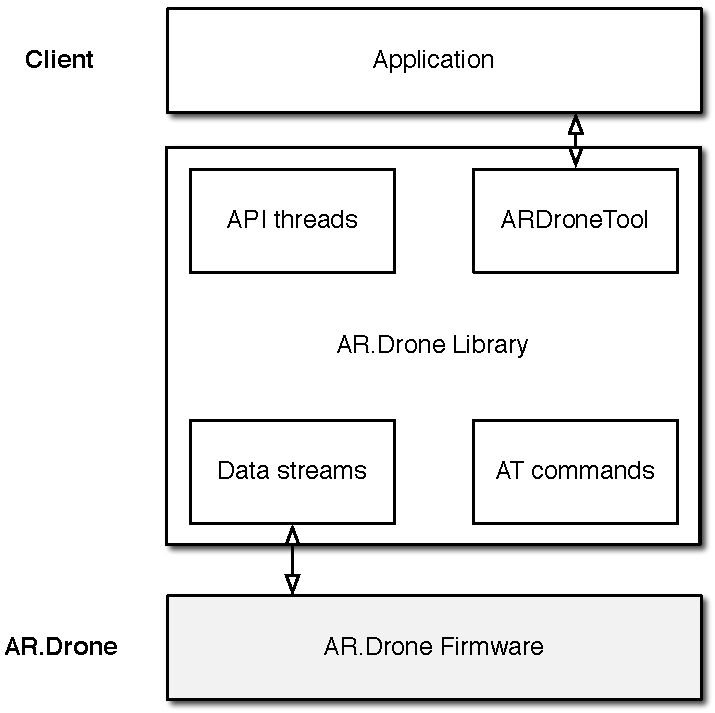
\includegraphics[height=8cm]{images/platform_ardroneapi.pdf}
\caption{Layered architecture of a client application built upon the AR.Drone SDK.}
\label{fig:platform-ardroneapi}
\end{figure}

The \textit{AR.Drone Library} is part of the SDK and provides high level APIs to access the drone.
Its content can be summarized as following:
\begin{itemize}
\item \textit{SOFT}, includes header files describing the communication structures;
	\begin{itemize}
		\item \textit{ARDroneTool} a set of tools to easily manage the drone, e.g., communication initialization, input-device management, high-level drone control functions and navdata receiving and decoding system;
	\end{itemize}
\item \textit{VPSDK}, a set of general purpose libraries: video processing pieces, multiplatform wrappers for system-level functions, multiplatform wrappers for communication functions and helpers to manage video pipelines and threads;
\item \textit{VLIB}, the video processing library. It contains the functions to receive and decode the video stream.
\end{itemize}

Unfortunately, the AR.Drone API has some drawbacks.
The API was mainly developed for the iPhone application.
Support for other platforms (e.g., Linux and Windows) was added in an early release and not updated for a while.
In order to make recent versions of the API working under Windows, a significant amount of fixes is required.
Another drawback is the bulkiness.
The API consists of many files and lines of undocumented code.
This makes it difficult to comprehend what is happening inside the code.

For these reasons, custom software libraries have been released by developers.
ARDrone-Control-.NET\footnote{\url{https://github.com/shtejv/ARDrone-Control-.NET}} provides a .Net SDK for Windows.
Another developer has written a MeeGo\footnote{\url{http://www.developer.nokia.com/Community/Blogs/blog/kate-alholas-forum-nokia-blog/2010/12/23/ar-drone-with-meego}} application to control the AR.Drone on Nokia devices. The AR.Drone logic is written in C++.
Another interesting project is an Urbi driver\footnote{\url{http://www.psykokwak.com/blog/}} in order to control and program the ARDrone from the Urbi platform.
Urbi is an open-source software platform to control robots or complex systems in general. The goal of Urbi is to help making robots compatible and simplify the process of writing programs and behaviors for those robots. 